%iffalse
\let\negmedspace\undefined
\let\negthickspace\undefined
\documentclass[journal,12pt,onecolumn]{IEEEtran}
\usepackage{cite}
\usepackage{amsmath,amssymb,amsfonts,amsthm}
\usepackage{algorithmic}
\usepackage{graphicx}
\usepackage{textcomp}
\usepackage{xcolor}
\usepackage{txfonts}
\usepackage{listings}
\usepackage{enumitem}
\usepackage{mathtools}
\usepackage{pgfplots}
\usepackage{gensymb}
\usepackage{comment}
\usepackage{circuitikz}
\usepackage[breaklinks=true]{hyperref}
\usepackage{tkz-euclide} 
\usepackage{listings}
\usepackage{gvv}                                        
%\def\inputGnumericTable{}                                 
\usepackage[latin1]{inputenc}                                
\usepackage{color}                                            
\usepackage{array}                                            
\usepackage{longtable}                                       
\usepackage{calc}                                             
\usepackage{multirow}                                         
\usepackage{hhline}                                           
\usepackage{ifthen}                                           
\usepackage{lscape}
\usepackage{tabularx}
\usepackage{array}
\usepackage{float}

\usepackage{enumitem}
\usepackage{xcolor}
%\usepackage{multicol}

\newtheorem{theorem}{Theorem}[section]
\newtheorem{problem}{Problem}
\newtheorem{proposition}{Proposition}[section]
\newtheorem{lemma}{Lemma}[section]
\newtheorem{corollary}[theorem]{Corollary}
\newtheorem{example}{Example}[section]
\newtheorem{definition}[problem]{Definition}
\newcommand{\BEQA}{\begin{eqnarray}}
\newcommand{\EEQA}{\end{eqnarray}}
\newcommand{\define}{\stackrel{\triangle}{=}}
\theoremstyle{remark}
\newtheorem{rem}{Remark}

\title{2020-AE-27-39}
\author{AI24BTECH11023 - Tarun Reddy Pakala}
\begin{document}
\bibliographystyle{IEEEtran}

\maketitle
\bigskip
\renewcommand{\thefigure}{\theenumi}
\renewcommand{\thetable}{\theenumi}
\begin{enumerate}
\item The positive high angle-of-attack condition is obtained in a steady pull-out maneuver at the largest permissible angle-of-attack of the wing. Under this condition, at which of the following regions of the wing does the maximum tension occur?
%input for figure 1
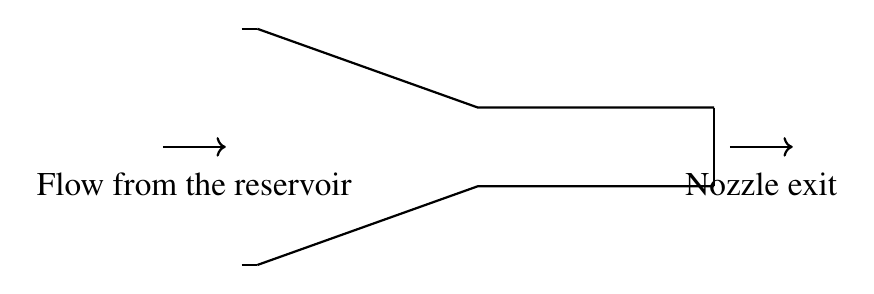
\begin{tikzpicture}
    % Draw the nozzle shape with short vertical lines at the opening
    \draw[thick] (-3,1.5) -- (-2.8,1.5);
    \draw[thick] (-3,-1.5) -- (-2.8,-1.5);
    \draw[thick] (-2.8,1.5) -- (0,0.5) -- (3,0.5);
    \draw[thick] (-2.8,-1.5) -- (0,-0.5) -- (3,-0.5);
    
    % Vertical line at the nozzle exit
    \draw[thick] (3,0.5) -- (3,-0.5);

    % Flow direction arrows
    \draw[->, thick] (-4,0) -- (-3.2,0);
    \draw[->, thick] (3.2,0) -- (4,0);

    % Labels for the flow and nozzle exit, placed below arrows
    \node[below] at (-3.6,-0.2) {\large Flow from the reservoir};
    \node[below] at (3.6,-0.2) {\large Nozzle exit};
\end{tikzpicture}

\begin{enumerate}
    \item $I$
    \item $II$
    \item $III$
    \item $IV$
\end{enumerate}
\item The natural frequency of the first mode of a rectangular cross section cantilever aluminum beam is $\omega \frac{rad}{s}$. If the material and cross-section remain the same, but the length of the beam is doubled, the first mode frequency will become
\begin{enumerate}
    \item $\frac{\omega}{4}\frac{rad}{s}$
    \item $4\omega \frac{rad}{s}$
    \item $\frac{\omega}{16} \frac{rad}{s}$
    \item $16\omega \frac{rad}{s}$
\end{enumerate}
\item Given $A=\begin{pmatrix}
    \sin \theta & \tan \theta \\
    0 & \cos \theta \\
\end{pmatrix}$, the sum of squares of eigenvalues of $A$ is
\begin{enumerate}
    \item $\tan^2\theta$
    \item $1$
    \item $\sin^2\theta$
    \item $\cos^2\theta$
\end{enumerate}
\item Burnout velocity of a space vehicle in a circular orbit at angle $5$ degrees above the local horizon around earth is $13.5\;\frac{km}{s}$. Tangential velocity of the space vehicle in the orbit is \underline{\hspace{2cm}} $\frac{km}{s}$ \brak{round\;off\;to\;two\;decimal\;places}.
\item Velocity of an airplane in the body fixed axes is given as $\sbrak{100\;-10\;20} \frac{m}{s}$. The sideslip angle is \underline{\hspace{2cm}} degrees \brak{round\;off \;to \;two\; decimal\; places}.
\item The similarity solution for the diffusion equation,$\frac{\partial u}{\partial t}=\alpha \frac{\partial^2u}{\partial x^2}$ is $u\brak{x,\;t}=u\brak{\eta}$, where similarity variable, $\eta=\frac{x}{\sqrt{\alpha t}}$. If $u\brak{x\;0}=e^{-x^2}$, the ratio $\frac{u\brak{0,\;1}}{u\brak{0\;4}}=$ \underline{\hspace{2cm}} \brak{round \; off \; to\; one \; decimal\;place }.
\item Air enters the rotor of an axial compressor stage with no pre-whirl \brak{C_\theta=0} and exits the rotor with whirl velocity, $C_\theta=150\frac{m}{s}$. The velocity of rotor vanes, $U$ is $200 \frac{m}{s}$. Assume $C_P=100\frac{J}{kg\;K}$, the stagnation temperature rise across the rotor is \underline{\hspace{2cm}} $K$ \brak{round\;off\;to\;one\;decimal\;place}.
\item A thin walled beam of constant thickness shown in the figure is subjected to a torque of $3.2\;kNm$. If the shear modulus is $25 GPa$, the angle of twist per unit length is \underline{\hspace{2cm}} $\frac{rad}{m}$ \brak{round\;off\;to\;three\;decimals}.
%input for figure 2
\begin{figure}[!ht]
\centering
\resizebox{3cm}{3cm}{%
\begin{circuitikz}
\tikzstyle{every node}=[font=\LARGE]
\draw [ line width=0.6pt](2.75,12) to[sinusoidal voltage source, sources/symbol/rotate=auto] (3.25,11.5);
\draw [ line width=0.6pt](3.25,11.75) to[european resistor] (9.5,11.75);
\draw [line width=0.6pt, ->, >=Stealth] (9.5,11.75) -- (9.5,11);
\draw [ line width=0.6pt](4,12.25) to[short] (4,11.25);
\draw [ line width=0.6pt](4,11.5) to[short] (4,11);
\draw [ line width=0.6pt](8.75,12.25) to[short] (8.75,11);
\draw [ line width=0.6pt](4,11.25) to[short] (4.5,11.25);
\draw [ line width=0.6pt](8.75,11.25) to[short] (8.25,11.25);
\draw [ line width=0.6pt](4.25,11.25) to[short] (5.25,11.25);
\draw [ line width=0.6pt](8.25,11.25) to[short] (7.25,11.25);
\draw [ line width=0.6pt](5,11.25) to[european resistor] (5,8.5);
\draw [ line width=0.6pt](7.5,11.25) to[european resistor] (7.5,8.5);
\draw [ line width=0.6pt](4.75,8.5) to[short] (8,8.5);
\draw [line width=0.6pt, ->, >=Stealth] (6.25,8.5) -- (6.25,7.75);
\node [font=\normalsize] at (6.75,8) {Bus 3};
\node [font=\normalsize] at (4,12.5) {Bus 1};
\node [font=\normalsize] at (8.75,12.5) {Bus 2};
\node [font=\normalsize] at (6.25,12.25) {j q};
\node [font=\normalsize] at (4.5,10) {j r};
\node [font=\normalsize] at (8.25,9.75) {j p};
\end{circuitikz}
}%

\label{fig:my_label}
\end{figure}

\item An airplane of mass $5000\;kg$ is flying at a constant speed of $360\;\frac{km}{h}$ at the bottom of a vertical circle with a radius of $400\;m$, as shown in the figure. Assuming that the acceleration due to gravity is $9.8\;\frac{m}{s^2}$, the load factor experienced at the center of gravity of the airplane is \underline{\hspace{2cm}} \brak{round\;off\;to\;two\;decimal\;places}. 
%input for figure 3
\begin{figure}[!ht]
\centering
\resizebox{3cm}{3cm}{%
\begin{circuitikz}
\tikzstyle{every node}=[font=\small]
\draw (4.25,12.25) to[battery1] (4.25,7.75);
\draw (4.25,12.25) to[short] (6.25,12.25);
\draw (4.25,7.75) to[short] (6.25,7.75);
\draw (6.25,12.25) to[R] (6.25,10.25);
\draw (6.25,10.25) to[R] (6.25,7.75);
\draw (6.25,10.25) to[short] (8.75,10.25);
\draw (6.25,7.75) to[short] (8.75,7.75);
\draw (8.75,7.75) to[R] (8.75,9.25);
\draw (8.75,10.25) to[D] (8.75,9);
\node [font=\small] at (4,10.25) {+};
\node [font=\small] at (4,9.75) {-};
\node [font=\small] at (4.75,10.5) {24 Volt};
\node [font=\small] at (6.75,11.25) {12 k$\Omega$};
\node [font=\small] at (6.75,9) {6 k$\Omega$};
\node [font=\small] at (8,8.5) {3.3 k$\Omega$};
\end{circuitikz}
}%

\label{fig:my_label}
\end{figure}

\item The equation $x\frac{dx}{dy}+y=c$, where $c$ is a constant, represents a family of
\begin{enumerate}
    \item exponential curves 
    \item parabolas 
    \item circles
    \item hyperbolas
\end{enumerate}
\item A wedge shaped airfoil is placed in a supersonic flow as shown in figure \brak{\text{not to scale}}. The corners of the wedge are at $x=\text{x}_A$, $x=\text{x}_B$,\;$x=\text{x}_C$, respectively.\\
%input for figure 4
\begin{figure}[H]
\centering
\resizebox{3cm}{3cm}{%
\begin{circuitikz}
\tikzstyle{every node}=[font=\small]
\draw [->, >=Stealth] (3.5,10.75) -- (3.5,13.75);
\draw [->, >=Stealth] (3.5,10.75) -- (10.75,10.75);
\draw [->, >=Stealth] (2.25,10.75) -- (3.25,10.75);
\draw [dashed] (4.5,13.25) -- (4.5,8.25);
\draw [dashed] (7.25,13.25) -- (7.25,8.25);
\draw [dashed] (10,13.25) -- (10,8.25);
\draw [dashed] (2,8.25) -- (10,8.25);
\draw [dashed] (2,13) -- (10,13);
\draw [short] (4.5,10.75) -- (7.25,11.75);
\draw [short] (7.25,11.75) -- (10,9.75);
\draw [short] (4.5,10.75) -- (10,9.75);
\node [font=\small] at (2.5,11) {$M>1$};
\node [font=\small] at (3.5,14) {$y$};
\node [font=\small] at (11,10.75) {$x$};
\node [font=\small] at (4.5,8) {$X_A$};
\node [font=\small] at (7.25,8) {$X_B$};
\node [font=\small] at (10,8) {$X_C$};
\node [font=\small] at (1.75,8.25) {$Y_{II}$};
\node [font=\small] at (1.75,13) {$Y_I$};
\node [font=\small] at (5.5,11) {$\alpha$};
\node [font=\small] at (6.5,10.5) {$\alpha$};
\node [font=\small] at (9,10) {$2\alpha$};
\end{circuitikz}
}%
\label{fig:my_label}
\end{figure}

Which one of the following represents the correct static pressure along $y=\text{Y}_I$ and $y=\text{Y}_{II}$?
\begin{enumerate}
    \item 
    %input for figure 5
\begin{figure}[!ht]
\centering
\resizebox{3cm}{3cm}{%
\begin{circuitikz}
\tikzstyle{every node}=[font=\small]
\draw [line width=0.6pt, short] (4,10.75) -- (8.25,10.75);
\draw [line width=0.6pt, short] (8.25,10.75) -- (9.75,12);
\draw [line width=0.6pt, short] (8.25,10.25) -- (9.75,11.5);
\draw [line width=0.6pt, short] (8.25,10.25) -- (9.75,9.25);
\draw [line width=0.6pt, short] (4,9.75) -- (8.25,9.75);
\draw [line width=0.6pt, ->, >=Stealth] (9.75,11.75) -- (10.25,12.25);
\draw [line width=0.6pt, ->, >=Stealth] (9.5,9) -- (10,8.5);
\draw [line width=0.6pt, ->, >=Stealth] (3.75,10.25) -- (5,10.25);
\node [font=\small] at (3.5,10.25) {$Q$};
\node [font=\small] at (10.5,12.5) {$Q_1$};
\node [font=\small] at (10.25,8.25) {$Q_2$};
\draw [line width=0.6pt, short] (8.25,9.75) -- (9.25,9);
\end{circuitikz}
}%

\end{figure}

    \item 
    %input for figure 6
\begin{figure}[H]
\centering
\resizebox{3cm}{3cm}{%
\begin{circuitikz}
\tikzstyle{every node}=[font=\large]
\draw [ line width=0.6pt ] (5.5,12.5) rectangle (7.5,6.25);
\draw [line width=0.6pt, dashed] (6.5,12.5) -- (6.5,6.25);
\draw [line width=0.6pt, dashed] (4.75,12.5) -- (8.5,12.5);
\draw [line width=0.6pt, dashed] (4.75,12.75) -- (8.5,12.75);
\draw [line width=0.6pt, dashed] (4.75,13) -- (8.5,13);
\draw [line width=0.6pt, dashed] (4.75,13.25) -- (8.5,13.25);
\draw [line width=0.6pt, dashed] (4.75,13.5) -- (8.5,13.5);
\draw [line width=0.6pt, ->, >=Stealth] (4.5,10.5) -- (4.5,8.75);
\draw [line width=0.6pt, <->, >=Stealth] (8.5,12.5) -- (8.5,6.25);
\node [font=\large] at (4,9.75) {$g$};
\node [font=\large] at (9.25,9.5) {L};
\end{circuitikz}
}%

\label{fig:my_label}
\end{figure}

    \item 
    %input for figure 7
 \begin{figure}[H]
\centering
\resizebox{3cm}{3cm}{%
\begin{circuitikz}
\tikzstyle{every node}=[font=\small]
\draw [line width=1.4pt, short] (8,13) -- (8,7.25);
\draw [line width=0.6pt, short] (3,7.25) -- (10.5,7.25);
\draw [line width=0.6pt, short] (3,7.25) -- (3,13);
\draw [line width=0.6pt, short] (3,12.75) -- (8,12.75);
\draw [line width=0.6pt, short] (3,10.75) -- (8,10.75);
\draw [line width=0.6pt, <->, >=Stealth] (3.75,12.75) -- (3.75,10.75);
\draw [line width=0.6pt, <->, >=Stealth] (3.75,10.75) -- (3.75,7.25);
\draw [line width=0.6pt, ->, >=Stealth] (8.75,11.75) -- (8.75,10.75);
\node [font=\small] at (3.25,11.75) {$1\; m$};
\node [font=\small] at (3.25,9) {$2\;m$};
\node [font=\small] at (5.5,11.75) {$1000\; \frac{kg}{m^3}$};
\node [font=\small] at (5.5,9) {$2000 \;\frac{kg}{m^3}$};
\node [font=\small] at (6,6.5) {Not to scale};
\node [font=\small] at (9,11.25) {$g$};
\node [font=\small] at (9,13) {$P_a$};
\node [font=\small] at (5.25,13.25) {$P_a$};
\node [font=\Huge] at (8,7.5) {.};
\draw [line width=0.6pt, ->, >=Stealth] (8.25,7.5) -- (8.75,8);
\node [font=\small] at (9.25,8.25) {Hinge};
\end{circuitikz}
}%

\label{fig:my_label}
\end{figure}

    \item 
    %input for figure 8
    \begin{figure}[H]
\raggedright
\resizebox{3cm}{3cm}{%
\begin{circuitikz}
\tikzstyle{every node}=[font=\small]
\draw [->, >=Stealth] (0.5,8) -- (0.5,12.5);
\draw [->, >=Stealth] (0.5,8) -- (6.5,8);
\draw [->, >=Stealth] (7,8) -- (13.25,8);
\draw [->, >=Stealth] (7,8) -- (7,12.5);
\draw [dashed] (1,12) -- (1,8.5);
\draw [dashed] (3,12) -- (3,8.75);
\draw [dashed] (5,12) -- (5,8.5);
\draw [short] (0.5,9.5) -- (1,9.5);
\draw [short] (1,9.5) -- (1,11.5);
\draw [short] (1,11.5) -- (3.5,11.5);
\draw [short] (3.5,11.5) -- (4.25,9.25);
\draw [short] (4.25,9.25) -- (5,9.25);
\draw [dashed] (7.5,12.25) -- (7.5,8.75);
\draw [dashed] (9.5,12.25) -- (9.5,8.75);
\draw [dashed] (12,12.25) -- (12,9);
\node [font=\small] at (8.5,12) {$Y_{II}$};
\node [font=\small] at (7.5,8.5) {$X_A$};
\node [font=\small] at (9.5,8.5) {$X_B$};
\node [font=\small] at (12,8.75) {$X_C$};
\node [font=\small] at (1,8.25) {$X_A$};
\node [font=\small] at (3,8.5) {$X_B$};
\node [font=\small] at (5,8.5) {$X_C$};
\node [font=\small] at (6.5,11.25) {P};
\node [font=\small] at (0.25,11.5) {P};
\node [font=\small] at (4,7.75) {$x$};
\node [font=\small] at (10.5,7.75) {$x$};
\node [font=\small] at (1.75,11.75) {$Y_I$};
\draw [short] (7,9.5) -- (8,9.5);
\draw [short] (8,9.5) -- (8,11.75);
\draw [short] (8,11.75) -- (12,11.75);
\end{circuitikz}
}%

\end{figure}

\end{enumerate}
\item The value of Poisson's ratio at which the shear modulus of an isotropic material is equal to the bulk modulus is
\begin{enumerate}
    \item $\frac{1}{2}$
    \item $\frac{1}{4}$
    \item $\frac{1}{6}$
    \item $\frac{1}{8}$
\end{enumerate}
\item A load P is applied to the free end of a stepped cantilever beam as shown in the figure. The Young's modulus of the material is $E$, and the moments of inertia of the two sections of length $2\;m$ and $1\;m$ are $I$ and $3I$, respectively. Ignoring transverse shear and stress concentration effects, the deflection at the point where the load is applied at the free end of the cantilever is  
%input for figure 9
\begin{figure}[!ht]
\centering
\resizebox{3cm}{3cm}{%
\begin{circuitikz}
\tikzstyle{every node}=[font=\small]
\draw [->, >=Stealth] (7.5,8.25) -- (7.5,12.5);
\draw [dashed] (5.25,10.25) -- (10,10.25);
\node [font=\small] at (5.5,9.5) {medium2};
\node [font=\small] at (5.25,11.25) {medium-1};
\node [font=\small] at (9.25,10) {z=0};
\end{circuitikz}
}%

\label{fig:my_label}
\end{figure}

\begin{enumerate}
    \item $\frac{23}{243EI}$
    \item $\frac{1}{3EI}$
    \item $\frac{43}{3EI}$
    \item $\frac{23}{3EI}$
\end{enumerate}


\end{enumerate}
\end{document}
